% Definition der Klasse des Dokumentes
\documentclass[11pt, a4paper]{article}

\usepackage[T1]{fontenc}        % Sorgt u.a. dafür, dass Texte vernünftig markierbar werden auch bei Sonderzeichen
\usepackage{ae,aecompl} %bessere Schrift
\usepackage{gensymb}
\usepackage[ngerman]{babel}     % Deutsches Wörterbuch usw.
\usepackage{epstopdf}   % Wandelt .eps Dateien automatisch um
\usepackage{url}    % für URL mit \url{.....}
\usepackage[font=small,labelfont=bf]{caption}       % Optionen für Bild- und Codeunterschriften
\usepackage[hidelinks]{hyperref}                    % damit Links in der PDF anklickbar werden
\usepackage{booktabs}   % bessere Tabellen mit Abstand zur hline
\pagenumbering{arabic}
\usepackage[babel,german=guillemets]{csquotes} %deutsches Anführungszeichen
\usepackage{float} %bessere Positionierungsoptionen

% Standardpakete für deutsche Sprache
\usepackage[utf8]{inputenc}
\usepackage[ngerman]{babel}

% Volle Seite nutzen
\usepackage{fullpage} 
\headsep 1cm
\parindent 0cm

% einige Pakete für Mathematische Darstellung
\usepackage{amssymb, amstext, amsmath}
\usepackage{fancyhdr}

% ein Paket für die Zählung von Seiten
\usepackage{count1to}
\usepackage{lastpage} 

%Paket für Aufzählungsbuchstaben
\usepackage{enumitem}


\usepackage{nameref}



% HIER DIE NAMEN UND EMAIL ANPASSEN
\def \ATutantName{Moritz Breipohl}
\def \ATutantEmail{mbreipohl@techfak.uni-bielefeld.de}
\def \BTutantName{Markus Rothgänger}
\def \BTutantEmail{mrothgaenger@techfak.uni-bielefeld.de}
% HIER DIE VERSUCHSNUMMER ANPASSEN
\def \Versuchsnummer{Versuch 4}
% HIER DIE GRUPPENNUMMER ANPASSEN
\def \Gruppennummer{Gruppe 5}
% HIER DEN TUTORNAMEN ANPASSEN
\def \Tutorname{Lukas Schmidt, Robin Ewers}

% Kopfzeile und Fußzeile
\lhead{\Versuchsnummer}
\chead{\textbf{Digitalelektronisches Praktikum}}
\rhead{\today}
\lfoot{\Gruppennummer}
\rfoot{\thepage\ von \pageref{LastPage}}
\cfoot{}

% Wird zur Einbindung von Bildern benötigt
\usepackage{graphicx}
\graphicspath{{images/}}

% Physikalische Einheiten darstellen
\usepackage{siunitx}

% Einbinden des Literaturverzeichnisses
\usepackage[style=numeric-comp]{biblatex}
\bibliography{literatur.bib}

% Wird zum Einbinden von LaTeX Code benötigt
\usepackage{color}
\usepackage{showexpl}
\lstset
{
    language=[LaTeX]TeX,
    breaklines=true,
    basicstyle=\tt\scriptsize,
    keywordstyle=\color{blue},
    identifierstyle=\color{magenta},
}

\renewcommand{\footrulewidth}{0.4pt}
\pagestyle{fancy}

% Konfiguration des Deckblatts
\begin{titlepage}
\title{\textbf{Digitalelektronisches Praktikum\\ Versuch 4}}
\author{\ATutantName \\ \emph{\ATutantEmail} \and \BTutantName\\ \emph{\BTutantEmail}}
\date{\Gruppennummer \\[3ex] Tutor: \Tutorname \\[3ex] \today}
\end{titlepage}

\begin{document}
% Einfügen des Deckblatts
\clearpage
\maketitle
\thispagestyle{empty}
\newpage

%%%%%%%%%%%%%%%%%%%%%%%%%%%%%%%%%%%%%%%%%
%%% Ab hier Beginn des Laborberichts: %%%%%%%%%%%%%%%%%%%%%

\section*{Versuchsaufbau}
\subsection*{Aufgabe}
In diesem Versuch war es Ziel, die Vor- und Nachteile von drei Verschiedenen Inverterschaltungen zu untersuchen. Dazu wurden die Schaltungen zum einen am Computer simuliert und zum anderen auf dem Steckbrett aufgebaut und gemessen. Hier sollten die Unterschiede aus Simulation und Messung herausgestellt werden.
\subsection*{Erwartung}
Erwartet wurde, dass alle Inverterschaltungen ein ähnliches Verhalten zeigen, wobei der ideale Einsatz vom Szenario abhängt.
\subsection*{Aufbau}
Als Schaltungen wurde zuerst der Inverter mit Lastwiderstand aufgebaut (\autoref{aufbauLast}). Als zweites der Anreicherungsinverter (\autoref{aufbauAnreicherung}) und zuletzt der CMOS-Inverter (\autoref{aufbauCMOS}).
In allen Schaltungen waren zwei Spannungsquellen nötig. Die Versorgungsspannung wurde konstant gehalten wobei die Schaltspannung dem Eingang des Inverters entsprach. Als Ausgang ist die Masche am Kondensator zu betrachten.
\begin{figure}
    \centering
    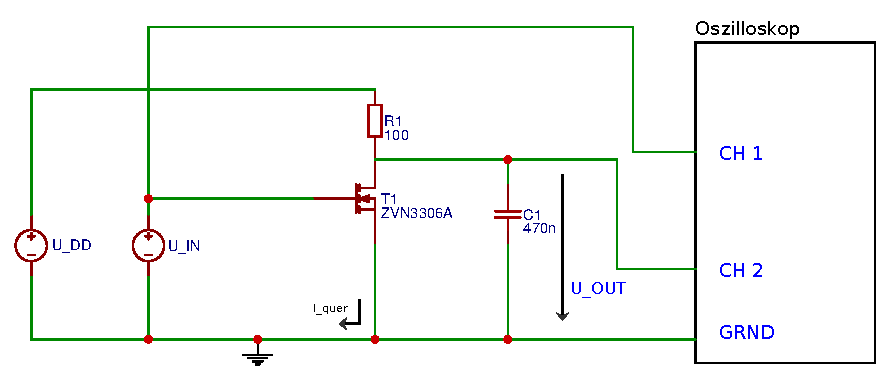
\includegraphics[width=\linewidth]{aufbauLast.pdf}
    \caption{Aufbau des Inverters mit Lastwiderstand}
    \label{aufbauLast}
\end{figure}
\begin{figure}
    \centering
    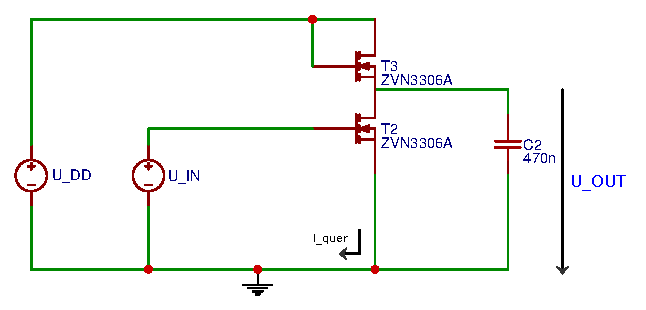
\includegraphics[width=\linewidth]{aufbauAnreicherung.pdf}
    \caption{Aufbau des Anreicherungsinverters}
    \label{aufbauAnreicherung}
\end{figure}
\begin{figure}
    \centering
    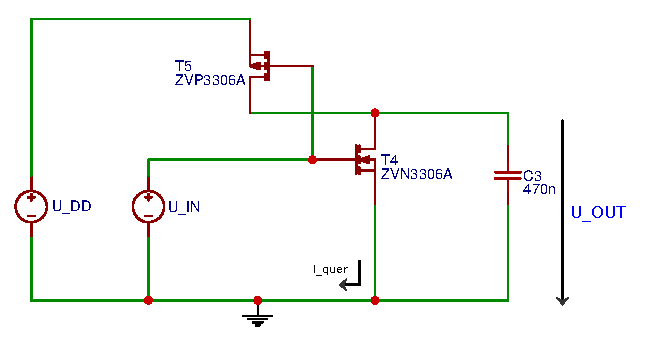
\includegraphics[width=\linewidth]{aufbauCMOS.pdf}
    \caption{Aufbau des CMOS-Inverters}
    \label{aufbauCMOS}
\end{figure}
Der Querstrom $I_{quer}$ wurde wie in den Schaltplänen eingezeichnet gemessen um Verlustströme aufzunehmen.
Um die Schaltzeit zu bestimmen, war des weiteren der Funktionsgenerator und das Oszilloskop nötig. Hier wurde der Funktionsgenerator anstelle der Eingangs-Stromversorgung eingebaut und der Ausgang am Kondensator über das Oszilloskop aufgenommen (exemplarisch im Schaltbild \autoref{aufbauLast} dargestellt).
\subsection*{Verwendete Bauteile}
Transistoren vom Typ ZVN3306A und ZVP3306A (nur CMOS-Inverter), Spannungsquellen mit begrenztem Strom, Multimeter, Kondensator mit einer Kapazität von $470 nF$, ein Widerstand mit $100 \Omega$ (nur Inverter mit Lastwiderstand), Funktionsgenerator und Oszilloskop (Schaltzeitmessung).
\section*{Durchführung Simulation}
Zuerst wurden die Schaltungen im Programm "LTSpice" aufgebaut und das Verhalten bzw. die Spannung am Ausgang bei einer Schrittweisen Erhöhung der Eingangsspannung ($U_{IN} = 0 V$ bis $U_{IN} = 5 V$) aufgenommen. Im zweiten Schritt wurde für jede Schaltung die Reaktions- bzw. Schaltzeit gemessen, indem die Eingangsspannung als Rechteckskurve simuliert wurde.
Die Ergebnisse wurde in Form von Datentabellen gesichert und anschließend geplottet. Die Versorgungsspannung wurde konstant auf $U_{DD} = 5 V$ gehalten.
\section*{Messergebnisse Simulation}
\begin{figure}
    \centering
    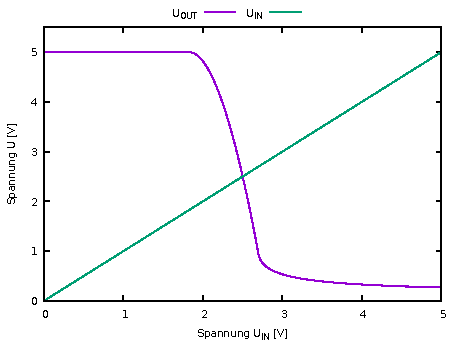
\includegraphics[width=\linewidth]{simLast.pdf}
    \caption{Schrittweise Erhöhung der Eingangsspannung \\ Inverter mit Lastwiderstand}
    \label{simLast}
\end{figure}
\begin{figure}
    \centering
    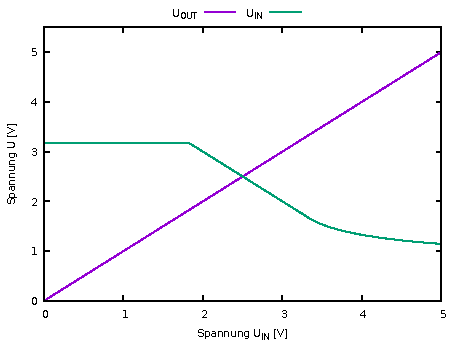
\includegraphics[width=\linewidth]{simAnreicherung.pdf}
    \caption{Schrittweise Erhöhung der Eingangsspannung \\ Anreicherungsinverter}
    \label{simAnreicherung}
\end{figure}
\begin{figure}
    \centering
    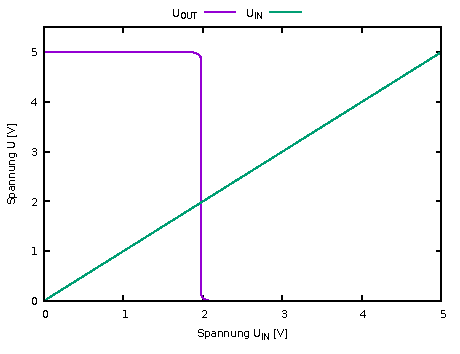
\includegraphics[width=\linewidth]{simCMOS.pdf}
    \caption{Schrittweise Erhöhung der Eingangsspannung \\ CMOS-Inverter}
    \label{simCMOS}
\end{figure}
Die Messergebnisse zum Verhalten beim Erhöhen der Eingangsspannung sind in \autoref{simLast} bis \autoref{simCMOS} dargestellt. 
Die Ergebnisse aus der Simulation zur Feststellung der Schaltzeit sind ebenfalls grafisch aufbereitet (\autoref{simTimeLast}  bis \autoref{simTimeCMOS}). Des weiteren wurden die Zeiten aus den Messdaten extrahiert, zu welchen die Ein- bzw. Ausgangsspannung auf die Hälfte der Amplitude gesunken bzw. gestiegen war. Aus diesen Daten wurde die Differenz gebildet (Schaltzeit). Die Ergebnisse sind in \autoref{simSchaltzeiten} zusammengefasst.
\begin{table}[h]
\centering
\begin{tabular}{c|c}
Inverter-Typ & Schaltzeit in ms \\ \hline
Lastwiderstand & $0.0284$ \\
Anreicherungstyp & $0.0024$ \\
CMOS & $0.0139$
\end{tabular}
\caption{Schaltzeiten nach Simulation der Invertertypen}
\label{simSchaltzeiten}
\end{table}
\begin{figure}
    \centering
    \includegraphics[width=\linewidth]{simTimeLast.pdf}
    \caption{Schaltzeitmessung in der Simulation \\ Inverter mit Lastwiderstand}
    \label{simTimeLast}
\end{figure}
\begin{figure}
    \centering
    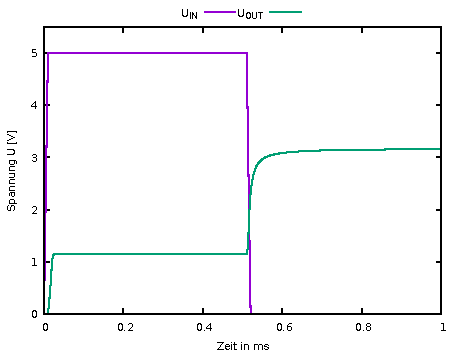
\includegraphics[width=\linewidth]{simTimeAnreicherung.pdf}
    \caption{Schaltzeitmessung in der Simulation \\ Anreicherungsnverter}
    \label{simTimeAnreicherung}
\end{figure}
\begin{figure}
    \centering
    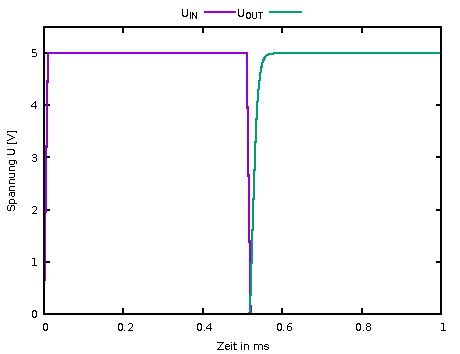
\includegraphics[width=\linewidth]{simTimeCMOS.pdf}
    \caption{Schaltzeitmessung in der Simulation \\ CMOS-Inverter}
    \label{simTimeCMOS}
\end{figure}
\section*{Durchführung Messung}
Ähnlich wie in der Simulation wurde bei der Messung am Steckbrett zunächst die Eingangsspannung schrittweise von null bis fünf Volt erhöht. 
Zur Messung der Schaltzeiten wurde eine vom Funktionsgenerator generierte Rechteckskurve mit einer Amplitude von $5V$ genutzt und die Eingangsspannung mit der Ausgangsspannung am Oszilloskop verglichen wobei die Schaltzeit mithilfe der Cursor gemessen wurde.
Die Versorgungsspannung blieb konstant bei fünf Volt.
\section*{Messergebnisse Messung}
\begin{table}[h]
\centering
\begin{tabular}{c|c}
Inverter-Typ & Schaltzeit in ms \\ \hline
Lastwiderstand & $0$ \\
Anreicherungstyp & $0$ \\
CMOS & $0$
\end{tabular}
\caption{Schaltzeiten nach Messung der Invertertypen}
\label{mesSchaltzeiten}
\end{table}
Die mit dem Oszilloskop bestimmten Schaltzeiten sind in \autoref{mesSchaltzeiten} dargestellt.
\subsection*{Beobachtungen}
Bei der Bestimmung der Schaltzeiten in der Simulation ist auffällig, dass die Schaltzeit für den Anreicherungsinverter im Vergleich sehr niedrig ist. Hier ist jedoch ebenfalls in Betracht zu ziehen, dass die Spannungsdifferenz der beiden Zustände gerade einmal $2 V$ beträgt. Bei den restlichen Schaltungen beträgt die Differenz volle $5V$.
\section*{Auswertung}
\section*{Literaturverzeichnis}
\end{document}
